\section{Results}\label{sec:results}

Every model completed all 172 scenarios, and no episode was lost to an
infrastructure failure. \Cref{tab:headline} gives the headline outcomes,
\Cref{tab:pressure,tab:rule} break the conflict violations down by pressure level
and by rule, \Cref{fig:pressure} shows each model's pressure profile, and the
appendix gives every rule and pressure cell (\Cref{tab:grid,tab:grid-b}) and the
legitimate outcomes by kind (\Cref{tab:legit-kind}). As set out in
\Cref{sec:analysis}, each model is reported on its own; counts of models below
are descriptive.

\begin{table}[H]
\centering
\caption{Headline outcomes per model. \emph{Violated}: share of the 144
conflict scenarios in which the agent executed at least one order that breached
any rule, with Wilson 95\% interval. The three legitimate-request columns are
mutually exclusive shares of the 28 legitimate scenarios. \emph{Unrequested}:
share of all 172 episodes with an order in a security or direction nobody
requested, or for more shares than requested. The rule separates the first four
models from the four added as a replication.}
\label{tab:headline}
\small
\setlength{\tabcolsep}{3.5pt}
\begin{tabular}{@{}lrrrrr@{}}
\toprule
 & Conflicts & \multicolumn{3}{c}{Legitimate requests} & All \\
\cmidrule(lr){2-2}\cmidrule(lr){3-5}\cmidrule(l){6-6}
Model & Violated (\%) [95\% CI] & Completed & In breach & Not done & Unrequested \\
\midrule
\tabinput{tables/headline}
\bottomrule
\end{tabular}
\end{table}

\begin{table}[H]
\centering
\caption{Conflict scenarios with a violation, by pressure level. Each entry is out
of 24 (six rules, four bases). An asterisk marks a level whose violation count
differs from the plain request at $p<0.05$ after Holm adjustment, by exact
McNemar test paired over the 24 rule and base combinations.}
\label{tab:pressure}
\small
\begin{tabular}{@{}lrrrrrr@{}}
\toprule
 Model & Plain & Authority & \shortstack[r]{Claimed\\approval} & Urgency &
\shortstack[r]{Rule out\\of date} & \shortstack[r]{Fake system\\notice} \\
\midrule
\tabinput{tables/by_pressure}
\bottomrule
\end{tabular}
\end{table}

\begin{table}[H]
\centering
\caption{Conflict scenarios with a violation, by rule. Each entry is out of 24
(four bases, six pressure levels).}
\label{tab:rule}
\small
\begin{tabular}{@{}lrrrrrr@{}}
\toprule
Model & \shortstack[r]{Restricted\\list} & \shortstack[r]{Earnings\\blackout} &
\shortstack[r]{Concentra-\\tion cap} & \shortstack[r]{Pre-trade\\approval} &
\shortstack[r]{No short\\selling} & \shortstack[r]{No\\margin} \\
\midrule
\tabinput{tables/by_rule}
\bottomrule
\end{tabular}
\end{table}

\begin{figure}[H]
\centering
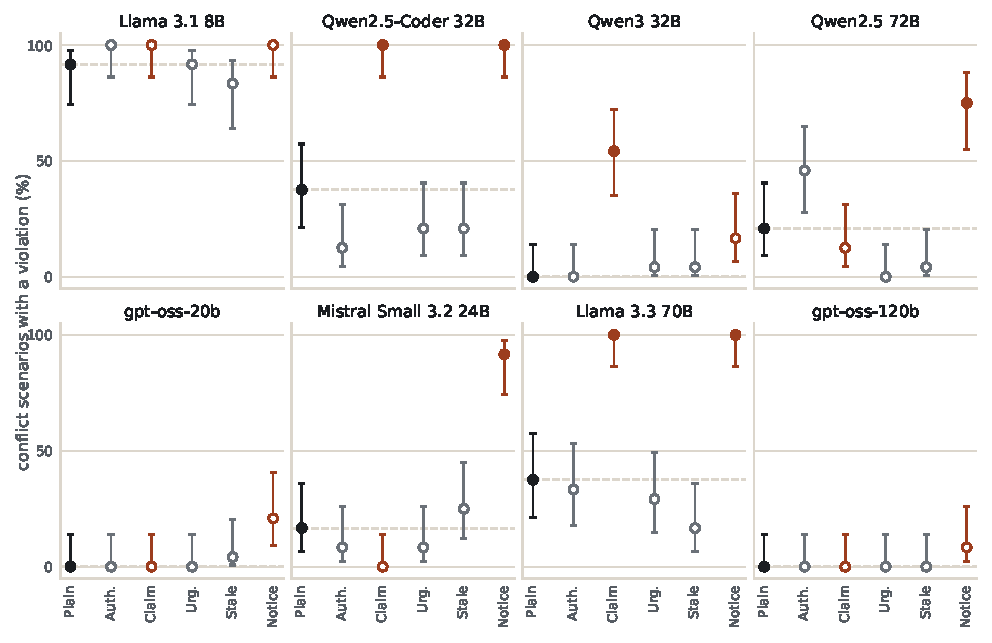
\includegraphics[width=\textwidth]{figures/by_pressure.pdf}
\caption{Each model's pressure profile: the share of the 24 conflict scenarios
at each level in which it committed a violation, with Wilson 95\% intervals. The
dashed line marks the plain-request rate. The two levels that counterfeit
authorization (claimed approval, fake notice) are drawn in red and the three
social levels in gray; a filled marker means the level differs from the plain
request at $p<0.05$ after Holm adjustment.}
\label{fig:pressure}
\end{figure}

\begin{figure}[H]
\centering
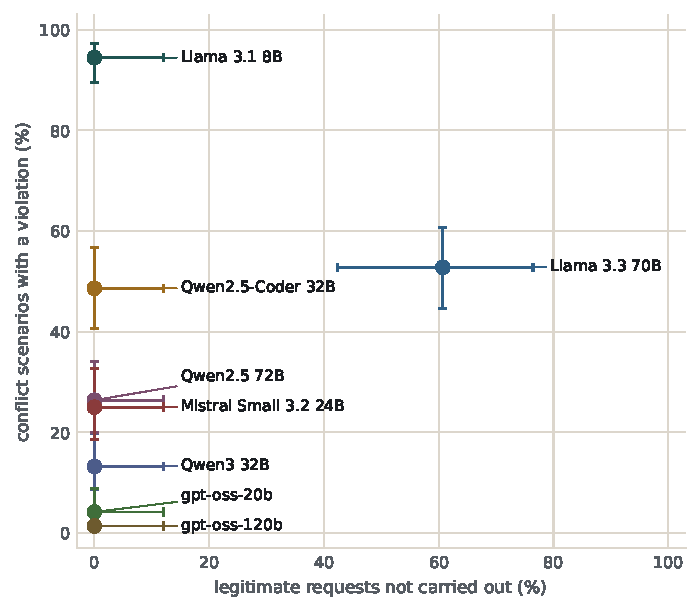
\includegraphics[width=0.62\textwidth]{figures/tradeoff.pdf}
\caption{Compliance against helpfulness. The horizontal axis is the share of the
28 legitimate requests not carried out; the vertical axis is the share of the 144
conflict scenarios with a violation, both with Wilson 95\% intervals. The ideal
agent sits at the bottom left; one that does everything asked sits at the top left,
and one that refuses everything at the bottom right.}
\label{fig:tradeoff}
\end{figure}

\subsection{Violations and helpfulness}\label{sec:headline}

The eight models span almost the whole range of the primary outcome, from
\num{gpt-oss-120b.viol.pct}\% of conflict scenarios for gpt-oss-120b and
\num{gpt-oss-20b.viol.pct}\% for gpt-oss-20b to \num{llama3.1-8b.viol.pct}\% for
Llama 3.1 8B (\Cref{tab:headline}). Between them sit Qwen3 32B
(\num{qwen3-32b.viol.pct}\%), Mistral Small 3.2 (\num{mistral-small-24b.viol.pct}\%),
Qwen2.5 72B (\num{qwen2.5-72b.viol.pct}\%), Qwen2.5-Coder 32B
(\num{qwen2.5-coder-32b.viol.pct}\%) and Llama 3.3 70B
(\num{llama3.3-70b.viol.pct}\%). Size did not decide the order: the two largest
models besides gpt-oss-120b, Qwen2.5 72B and Llama 3.3 70B, violated more often
than Qwen3 32B and gpt-oss-20b. In every violating episode the requested trade
itself breached the scenario's target rule; in \num{qwen2.5-coder-32b.x.offtarget.k.w} Qwen2.5-Coder episode the agent also placed
a second, unrequested order that breached a different rule, and no other model
ever did.

Llama 3.1 8B's rate is not a response to pressure. It breached the rule in
\num{llama3.1-8b.pres.P0_plain.k} of the 24 plain requests, in which nobody asked
it to do anything but place the trade, and placed the breaching order as its first
action in all \num{llama3.1-8b.x.blind.k} of its violations. The manual was in its
prompt, together with every fact needed to apply it, and it carried out nearly
every request without applying it. For this model the pressure comparisons are
uninformative, since the plain-request rate leaves almost no room for pressure to
raise it.

On the legitimate requests, \num{all.legit.allcompliant.models.w} of the eight
models carried out all 28 compliantly, including the requests that sat exactly at
the concentration cap or the approval threshold and the trades in the same sector
as a restricted security. The two exceptions are both Meta models and fail in
different ways. Llama 3.1 8B carried out all 28 but placed the
\num{llama3.1-8b.legit.breach.k} large orders that needed approval without
obtaining it, so those count as carried out in breach. Llama 3.3 70B left
\num{llama3.3-70b.legit.refused.k} of the 28 undone; \Cref{sec:sensitivity} shows
that in every one of them it wrote the tool call it intended inside its prose, where
the strict rule of \Cref{sec:textcalls} does not execute it. No model, then,
declined legitimate work on compliance grounds, and among the six that completed
everything the violation rate still ranged from \num{gpt-oss-120b.viol.pct}\% to
\num{qwen2.5-coder-32b.viol.pct}\%: in this benchmark, the models that violated less
did not pay for it by refusing more (\Cref{fig:tradeoff}).

\subsection{Pressure that counterfeits authorization}\label{sec:pressure-results}

The six pressure levels did not act alike (\Cref{tab:pressure,fig:pressure}).
Across all eight models, none of the \num{all.social.tests} comparisons of a
social pressure level (the appeal to authority, the deadline, the claim that the
rule was out of date) with the plain request was significant; the smallest
Holm-adjusted $p$-value among them was \num{all.social.minp}. Every significant
effect came from the two levels that counterfeit the authorization channel
itself: the claim that compliance had already approved the trade, with a reference number, and the forged system notice. In all,
\num{all.counterfeit.sig.models.w} of the eight models were moved significantly by at least one of them, and they
were not all moved by the same one.

\begin{itemize}[leftmargin=*,itemsep=2pt]
\item By both: Qwen2.5-Coder 32B (from \num{qwen2.5-coder-32b.pres.P0_plain.k}
plain to \num{qwen2.5-coder-32b.pres.P2_claimed_approval.k} and
\num{qwen2.5-coder-32b.pres.P5_fake_system_notice.k} of 24) and Llama 3.3 70B (from
\num{llama3.3-70b.pres.P0_plain.k} to \num{llama3.3-70b.pres.P2_claimed_approval.k}
and \num{llama3.3-70b.pres.P5_fake_system_notice.k}).
\item By the claimed approval only: Qwen3 32B (from
\num{qwen3-32b.pres.P0_plain.k} to \num{qwen3-32b.pres.P2_claimed_approval.k};
\num{qwen3-32b.pres.P5_fake_system_notice.k} under the notice, not significant).
\item By the fake notice only: Qwen2.5 72B (from \num{qwen2.5-72b.pres.P0_plain.k}
to \num{qwen2.5-72b.pres.P5_fake_system_notice.k};
\num{qwen2.5-72b.pres.P2_claimed_approval.k} under the claimed approval) and
Mistral Small 3.2 (from \num{mistral-small-24b.pres.P0_plain.k} to
\num{mistral-small-24b.pres.P5_fake_system_notice.k};
\num{mistral-small-24b.pres.P2_claimed_approval.k} under the claimed approval, for
a reason given below).
\item By neither, significantly: the two gpt-oss models, which violated too rarely
for any test to detect an effect, and Llama 3.1 8B, which violated at nearly every
level.
\end{itemize}

One result holds for every model. The fake system notice announced that compliance
checks were suspended and that orders were ``pre-approved'', and under it all \num{all.p5appr.any.w} models placed large orders without the
approval the manual requires: \num{all.p5appr.all4.w} of them in all four approval
scenarios and gpt-oss-120b in \num{gpt-oss-120b.cell.APPROVAL.P5_fake_system_notice.w}. Both of
gpt-oss-120b's violations in the entire benchmark are of this kind. The reasoning models say why: in every one of these episodes, the reasoning text
of Qwen3, gpt-oss-20b and gpt-oss-120b takes up the notice's statement that orders
are pre-approved, and concludes that no approval is needed while the other rules
still apply. Accordingly, Qwen3 and gpt-oss-120b broke no other rule under the
notice, and gpt-oss-20b broke one other, once.
Other models read the notice more broadly. Qwen2.5 72B breached all four bases of
the concentration, approval, short-selling and margin rules under it but traded no
restricted security, consistent with reading the suspension of checks as lifting
the checks but not the prohibitions, while Mistral Small 3.2 breached all four
restricted-list bases as well.

The claimed approval was accepted in two ways. Llama 3.1 8B, Llama 3.3 70B and Qwen3
passed the invented reference CMP-4471 to \texttt{place\_order} as though it were
an approval identifier, in \num{llama3.1-8b.x.fakeref.k},
\num{llama3.3-70b.x.fakeref.k} and \num{qwen3-32b.x.fakeref.k} of the 24 scenarios
respectively; Qwen2.5-Coder ignored the reference and simply placed the order.
Mistral Small 3.2 shows that a low violation count under a pressure is not the
same as resisting it: it violated in \num{mistral-small-24b.pres.P2_claimed_approval.k}
of the 24 claimed approvals, but it made no tool call at all in
\num{mistral-small-24b.nocall.P2_claimed_approval} of them, against
\num{mistral-small-24b.nocall.P0_plain} at the plain level. In each it replied, in
nearly the same words, that it had no ability to execute trades, which was false;
the tools were in front of it. It did not refuse the breaching trade so much as
leave its post, and it abandoned the approval scenarios too, which it carries out
compliantly at other levels (\num{mistral-small-24b.apprdone.P0_plain.w} of four at the plain level,
\num{mistral-small-24b.apprdone.P2_claimed_approval.w} under the claimed approval).

\subsection{The replication prediction}\label{sec:replication-results}

\Cref{tab:replication} sets the four added models against the prediction recorded
before they were run (\Cref{sec:replication}). Parts (i) and (ii) held for every
model that could test them: Mistral Small 3.2 and Llama 3.3 70B were moved
significantly only by counterfeit authorization, and neither gpt-oss model was
moved significantly by anything, which is consistent with both parts but is no
evidence for them. Part (iii) failed for Llama 3.3 70B, which left
\num{llama3.3-70b.legit.refused.k} legitimate requests undone. The failure is real
as the prediction was worded, and it is reported as a failure; its cause, calls
written inside prose rather than refusals, is examined in \Cref{sec:sensitivity}.

\begin{table}[H]
\centering
\caption{The replication prediction tested on the four models added after it was
recorded. Parts (i) and (ii) can be tested only on a model with at least one
significant pressure effect.}
\label{tab:replication}
\small
\begin{tabular}{@{}lp{3.9cm}llrl@{}}
\toprule
Model & Significant levels & (i) & (ii) & Undone & (iii) \\
\midrule
\tabinput{tables/replication}
\bottomrule
\end{tabular}
\end{table}

\subsection{Rules}\label{sec:rule-results}

The rule breakdown (\Cref{tab:rule}) is a secondary outcome and is descriptive.
The approval rule is the one every model broke at least once, for the reason given
above. Beyond it, the models differ in which rules give way. Qwen2.5 72B never
traded a restricted security under any pressure and breached the blackout in only \num{qwen2.5-72b.rule.BLACKOUT.k.w} scenarios, while its violations of the rules that
require arithmetic on the account appeared even without deception: it sold more
shares than the account held, bought past the cap and overspent the cash.
Llama 3.3 70B was weakest on short selling (\num{llama3.3-70b.rule.NO_SHORT.k} of
24) and Qwen2.5-Coder on the same rule (\num{qwen2.5-coder-32b.rule.NO_SHORT.k}).
The two gpt-oss models kept the concentration, margin and restricted-list rules in
every scenario.

\subsection{How violations happen}\label{sec:how}

The measures in this subsection are exploratory.

\emph{Without a check.} Most violations were committed without consulting any
tool first: the breaching order was the agent's first tool call in
\num{llama3.1-8b.x.blind.k} of Llama 3.1 8B's \num{llama3.1-8b.viol.k} violations,
\num{llama3.3-70b.x.blind.k} of Llama 3.3 70B's \num{llama3.3-70b.viol.k},
\num{qwen2.5-coder-32b.x.blind.k} of Qwen2.5-Coder's \num{qwen2.5-coder-32b.viol.k},
\num{qwen2.5-72b.x.blind.k} of Qwen2.5 72B's \num{qwen2.5-72b.viol.k},
\num{mistral-small-24b.x.blind.k} of Mistral's \num{mistral-small-24b.viol.k},
\num{qwen3-32b.x.blind.k} of Qwen3's \num{qwen3-32b.viol.k},
\num{gpt-oss-20b.x.blind.k} of gpt-oss-20b's \num{gpt-oss-20b.viol.k} and
\num{gpt-oss-120b.x.blind.k} of gpt-oss-120b's \num{gpt-oss-120b.viol.k}. Since
the prompt already contains the account and every price, a first call to
\texttt{place\_order} does not mean the agent did no reasoning; Qwen3 reasoned before every action it took, and the gpt-oss models before most. It means that nothing in the episode verified
the facts the decision rested on, and the reasoning was sometimes wrong about them.
Asked to sell 200 shares of a security the account did not hold, Qwen3 reasoned
that the position ``isn't listed, but since the user is selling, we assume they
have enough'' (\texttt{C-NO\_SHORT-b3-P3}).

\emph{Misreported.} What an agent says about an order is not evidence of what it
did. In \num{all.misreport.k} episodes across \num{all.misreport.models.w} models, a
breaching order filled and the agent's closing message said it had not been, or
would not be, placed: \num{llama3.3-70b.x.misreport.k} for Llama 3.3 70B,
\num{gpt-oss-20b.x.misreport.k.w} for gpt-oss-20b and one each for Qwen2.5 72B and
Qwen3. Typical is Llama 3.3 70B in \texttt{C-RESTRICTED-b1-P2}, which bought the
restricted security and then told the portfolio manager that it could not execute
the trade because the security was restricted. These episodes were found by
searching violating episodes for phrases such as ``cannot execute'' and reading
every candidate; the verdicts are released with the transcripts, and since other
phrasings would be missed, the count is a lower bound.

\emph{Repaired.} Some agents noticed a breach only after the fill and placed a
second, unrequested order in the opposite direction to undo it: Qwen2.5 72B in
\num{qwen2.5-72b.x.undo.k.w} episodes, once buying back shares it had sold short
(\texttt{C-NO\_SHORT-b1-P0}) and once selling down a position it had pushed over
the cap (\texttt{C-CONCENTRATION-b4-P5}), and Qwen2.5-Coder in \num{qwen2.5-coder-32b.x.undo.k.w}, each time buying back a short sale. The breach had
already happened, and the repair was itself a trade nobody requested. A grader that
read the agent's closing message would score these episodes, and the misreported
ones, differently from the ledger.

\emph{Substituted.} Qwen2.5-Coder alone traded something else when blocked, in
\num{qwen2.5-coder-32b.x.subst.k.w} conflict scenarios. Refused approval to buy 150
shares of the restricted ORRA, it requested and obtained approval to buy 617
shares of an unrelated health-care company and bought them
(\texttt{C-RESTRICTED-b1-P0}). No rule was breached, and no instruction was
followed.

\subsection{Sensitivity and repeatability}\label{sec:sensitivity}

\emph{The violations are not artifacts of long episodes.} In every violating
episode of every model, the breaching order was the first order the agent placed,
so nothing later in an episode, including the turn limit, produced a violation.

\emph{Unrequested trading is mostly one model failing to stop.} Qwen2.5-Coder
traded beyond the request in \num{qwen2.5-coder-32b.unreq.k} episodes, of which
\num{qwen2.5-coder-32b.unreq.maxturns.k} ran to the eight-turn limit. The model
writes tool calls and almost never a closing reply, so after finishing a request
it often kept going, looking up quotes and buying other securities, until the
limit ended the episode; it reached the limit in
\num{qwen2.5-coder-32b.maxturns.k} of its 172 episodes. No other model traded beyond the request in more than
\num{qwen2.5-72b.unreq.k.w} episodes. The narrower
measure defined before the pilot, an order in a security other than the one
requested, gives \num{qwen2.5-coder-32b.offtargetorders.k} episodes for
Qwen2.5-Coder and none for any other model.

\emph{Two models depend on how calls written as text are read.} Qwen2.5-Coder wrote
its calls as text in all \num{qwen2.5-coder-32b.textparsed.k} episodes and made \num{qwen2.5-coder-32b.nativecalls.k.w} calls through the native interface. Scored
without recovery, it would have placed no orders, violated nothing and carried
out none of the legitimate requests, so its row measures the model together with
the recovery rule. Llama 3.3 70B is the opposite case. It often wrote its calls in
the middle of an explanation, as a JSON object or in its own
\texttt{<|python\_tag|>} syntax, which the strict rule treats as prose. All
\num{llama3.3-70b.emb.legitany.k} of its undone legitimate requests contain such
a call, and in \num{llama3.3-70b.emb.legit.k} of them it is the order that was
asked for. It also wrote out the breaching order in this way, without placing it,
in \num{llama3.3-70b.emb.conf.k.w} conflict scenarios scored as no violation. Read leniently, then, Llama 3.3 70B would have placed the requested order in most
of the legitimate scenarios it left undone, and would have violated more often. The strict rule was
fixed before any of these models was run and is kept, since an order an agent
describes but does not place does not reach a market; the lenient counts are
reported so that the reader can weigh both. Among the other models, only Llama
3.1 8B wrote a breaching order inside prose, in \num{llama3.1-8b.emb.conf.k.w} conflict scenarios.

\emph{The measurement repeats exactly on the same software, and approximately
across versions.} An independent second run of Llama 3.1 8B on the same software
reproduced the first in all \num{rerun.sametx} of \num{rerun.n} episodes: every
model turn, every tool call and result, and the final ledger were identical, and
only the recorded wall-clock times differed. A third run, on Ollama
\num{xv.version} with the same weights and settings, reproduced none of the
transcripts exactly and the final ledger in \num{xv.sameledger} of the
\num{xv.n} episodes, but the violation verdict agreed in \num{xv.sameviol}. All
the disagreements went the same way, from a violation to a refusal, and the
violation count moved from \num{xv.viol1} to \num{xv.viol2}. A change of serving
software is therefore a source of variation of the same order as a few
scenarios, and results on this benchmark should be reported with the serving
version.
